% Drawing 82/02-1 -- folder 82, batch 02, archive page 33 (PDF page 34).
% Transcription: à droite, une figure : un cercle portant les points $\zeta_{-1}$, $\zeta_0$, $\zeta_1$, $\zeta_2$, $\zeta_3$, et plus haut à gauche $\zeta_{n-2}$ ; des flèches vont de $\zeta_{-1}$ à $\zeta_0$ (épaisse), de $\zeta_0$ à $\zeta_1$ ($e_1$), de $\zeta_1$ à $\zeta_2$ ($e_2$), de $\zeta_2$ à $\zeta_3$ ($e_3$), côtés successifs d'un polygone régulier inscrit, et une flèche épaisse marquée $\alpha$ va de $\zeta_0$ à $\zeta_3$.
% Kind: regular polygon inscribed in a circle, with side vectors and a diagonal. Method 2 (schematic redraw from the facsimile). Status: ok.
% Notes: A freehand circle of which he draws the arc from the right, over the top (where it carries a small brace-like kink), round the left down to zeta_0; the lower right part, where the polygon lies, is not closed, and it is left open here. The five consecutive vertices zeta_{-1}, zeta_0, zeta_1, zeta_2, zeta_3 are placed where they stand on the page (zeta_0 and zeta_1 inside the circle, the steps unequal); arrows along the four sides, the first heavy, the others labelled e_1, e_2, e_3; a heavy arrow alpha from zeta_0 to zeta_3, with a second, thinner arrow from zeta_0 half-way along it; the label zeta_{n-2} beside the upper left of the circle, with no point. The text says u is the rotation sending zeta_i to zeta_{i+1}, so the vertices are meant equally spaced; the page draws them freehand, and the redraw follows the page. Nothing struck; the foot of the half-sheet is torn below the figure. Overlaid 2026-11-12 (Opus 5.5) on a 400 dpi colour render: the earlier redraw put the vertices at equal steps on a fitted circle, up to 5 units from the page, with a circle too large and labels displaced; redrawn on the vertices, arc and labels measured on the page. Redrawn 2026-11-12 (issue 128): to check again.
% Coordinates: 1 unit = 1 mm = 1/100 of the crop width (bbox in page fractions: [0.63, 0.345, 0.87, 0.46]).
% Redrawn by Claude (claude-fable-5-2), issue #128, 2026-11-12; not checked by a human; not compiled (no TeX in the session).
% Overlaid by Claude (claude-opus-5-5) 2026-11-12 (issue #128): rasterised from its own coordinates over the colour facsimile and checked or corrected. Not compiled. Status: ok.
% Rights: reproduces part of the work -- behind RENDER_TRANSCRIPTS, never published by itself.
\documentclass[tikz,border=3pt]{standalone}
\usepackage{amsmath,amssymb}
\usetikzlibrary{patterns,arrows.meta}
\tikzset{pencil/.style={black!45}, struck/.style={black!35}, mpt/.style={circle,draw,inner sep=1.3pt}, pt/.style={circle,fill,inner sep=0.9pt}, opt/.style={circle,draw,fill=white,inner sep=1.1pt}}
\begin{document}
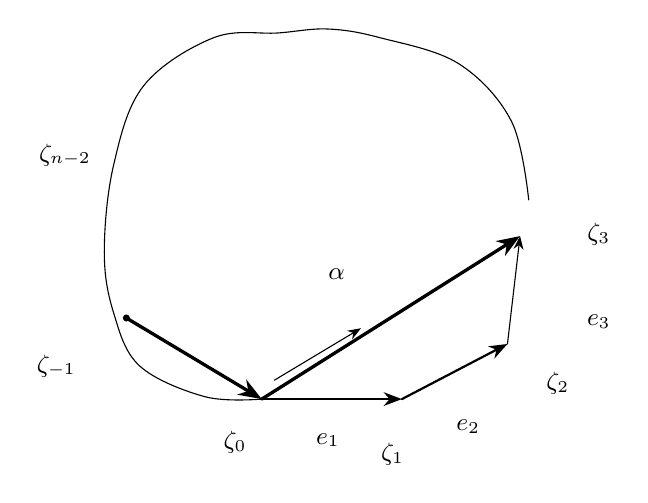
\begin{tikzpicture}[x=1mm,y=1mm,line cap=round,line join=round,font=\small]
\coordinate (zm) at (22.2,-41.7);
\coordinate (z0) at (39.4,-52);
\coordinate (z1) at (57.2,-52);
\coordinate (z2) at (70.6,-45);
\coordinate (z3) at (72.2,-31.3);
\draw plot[smooth, tension=0.6] coordinates {(73.3,-26.7) (71.1,-16.7) (64.4,-9.4) (54.4,-6.1) (47.8,-5) (41.5,-5.5) (33.3,-6.1) (24.4,-12.2) (20.6,-22.2) (19.4,-33.3) (20.6,-41.1) (23.9,-47.8) (32.2,-51.7) (z0)};
\draw[very thick,-{Stealth}] (zm) -- (z0);
\draw[thick,-{Stealth}] (z0) -- (z1);
\draw[thick,-{Stealth}] (z1) -- (z2);
\draw[-{Stealth}] (z2) -- (z3);
\draw[very thick,-{Stealth}] (z0) -- (z3);
\draw[-{Stealth}] (41,-49.6) -- (52,-43);
\node[pt] at (zm) {};
\node at (48.9,-36.1) {\small $\alpha$};
\node at (47.8,-57.2) {\small $e_1$};
\node at (65.6,-55.5) {\small $e_2$};
\node at (82.2,-42.2) {\small $e_3$};
\node at (13.3,-47.8) {\small $\zeta_{-1}$};
\node at (36,-57.5) {\small $\zeta_0$};
\node at (56,-59) {\small $\zeta_1$};
\node at (77,-50) {\small $\zeta_2$};
\node at (82.2,-31.1) {\small $\zeta_3$};
\node at (14.4,-21) {\small $\zeta_{n-2}$};
\end{tikzpicture}
\end{document}
